\documentclass[aspectratio=169,10pt]{beamer}

% ==============================================================================
% Modern Minimalist Beamer Theme for MLOps Architecture Defense
% ==============================================================================
\usetheme{default}
\useinnertheme{rectangles}
\usefonttheme{structurebold}

\usepackage[utf8]{inputenc}
\usepackage{helvet}
\renewcommand{\familydefault}{\sfdefault}
\usepackage{graphicx}
\usepackage{booktabs}
\usepackage{array}
\usepackage{ragged2e}
\usepackage{tikz}
\usetikzlibrary{shapes.geometric,arrows.meta,positioning,fit,calc,backgrounds,shadows.blur}
\usepackage{xcolor}
\usepackage[most]{tcolorbox}

% --- Modern Professional Color Palette ---
\definecolor{SlateDark}{HTML}{0F172A}    % Primary dark slate header
\definecolor{SlateMid}{HTML}{1E293B}     % Card border / secondary
\definecolor{SlateLight}{HTML}{F8FAFC}   % Card background fill
\definecolor{BlueAccent}{HTML}{2563EB}   % Vibrant engineering blue
\definecolor{GreenAccent}{HTML}{059669}  % Emerald success / verification
\definecolor{AmberAccent}{HTML}{D97706}  % Warm amber / telemetry / alert
\definecolor{RoseAccent}{HTML}{E11D48}   % Rose red / gatekeeper / danger
\definecolor{PurpleAccent}{HTML}{7C3AED} % Royal purple / active learning
\definecolor{TealAccent}{HTML}{0D9488}   % Teal / data engineering
\definecolor{TextMain}{HTML}{1E293B}     % Primary text
\definecolor{TextMuted}{HTML}{64748B}    % Secondary muted text

% --- Beamer Color Mappings ---
\setbeamercolor{normal text}{fg=TextMain,bg=white}
\setbeamercolor{structure}{fg=BlueAccent}
\setbeamercolor{frametitle}{fg=white,bg=SlateDark}
\setbeamercolor{title}{fg=white,bg=SlateDark}
\setbeamercolor{block title}{fg=white,bg=BlueAccent}
\setbeamercolor{block body}{fg=TextMain,bg=SlateLight}

% --- Clean Header / Footer Templates ---
\setbeamertemplate{navigation symbols}{}
\setbeamertemplate{headline}{}

\setbeamertemplate{frametitle}{%
    \nointerlineskip
    \begin{beamercolorbox}[wd=\paperwidth,ht=30pt,dp=7pt,leftskip=14pt,rightskip=14pt]{frametitle}
        {\large\bfseries\insertframetitle}
        \ifx\insertframesubtitle\@empty\else
            \\[2pt]{\footnotesize\color{TextMuted!40}\insertframesubtitle}
        \fi
    \end{beamercolorbox}
}

\setbeamertemplate{footline}{%
    \begin{beamercolorbox}[wd=\paperwidth,ht=14pt,dp=4pt,leftskip=14pt,rightskip=14pt]{normal text}
        {\tiny\color{TextMuted}\textbf{TaxonVision} $\cdot$ Production MLOps Architecture}
        \hfill
        {\tiny\color{TextMuted}\insertframenumber{} / \inserttotalframenumber}
    \end{beamercolorbox}
}

% --- Custom tcolorbox Card Environments ---
\newtcolorbox{card}[1][]{
    enhanced, colback=SlateLight, colframe=SlateMid!30,
    boxrule=0.5pt, arc=2.5pt, left=5pt, right=5pt, top=3pt, bottom=3pt,
    fontupper=\footnotesize\RaggedRight,
    fuzzy shadow={0.8pt}{-0.8pt}{0pt}{0.1pt}{black!8}, #1
}
\newtcolorbox{bluecard}[1][]{
    enhanced, colback=BlueAccent!5, colframe=BlueAccent!60,
    boxrule=0.5pt, arc=2.5pt, left=5pt, right=5pt, top=3pt, bottom=3pt,
    fontupper=\footnotesize\RaggedRight,
    fuzzy shadow={0.8pt}{-0.8pt}{0pt}{0.1pt}{black!8}, #1
}
\newtcolorbox{greencard}[1][]{
    enhanced, colback=GreenAccent!5, colframe=GreenAccent!60,
    boxrule=0.5pt, arc=2.5pt, left=5pt, right=5pt, top=3pt, bottom=3pt,
    fontupper=\footnotesize\RaggedRight,
    fuzzy shadow={0.8pt}{-0.8pt}{0pt}{0.1pt}{black!8}, #1
}
\newtcolorbox{ambercard}[1][]{
    enhanced, colback=AmberAccent!5, colframe=AmberAccent!60,
    boxrule=0.5pt, arc=2.5pt, left=5pt, right=5pt, top=3pt, bottom=3pt,
    fontupper=\footnotesize\RaggedRight,
    fuzzy shadow={0.8pt}{-0.8pt}{0pt}{0.1pt}{black!8}, #1
}
\newtcolorbox{rosecard}[1][]{
    enhanced, colback=RoseAccent!5, colframe=RoseAccent!60,
    boxrule=0.5pt, arc=2.5pt, left=5pt, right=5pt, top=3pt, bottom=3pt,
    fontupper=\footnotesize\RaggedRight,
    fuzzy shadow={0.8pt}{-0.8pt}{0pt}{0.1pt}{black!8}, #1
}
\newtcolorbox{purplecard}[1][]{
    enhanced, colback=PurpleAccent!5, colframe=PurpleAccent!60,
    boxrule=0.5pt, arc=2.5pt, left=5pt, right=5pt, top=3pt, bottom=3pt,
    fontupper=\footnotesize\RaggedRight,
    fuzzy shadow={0.8pt}{-0.8pt}{0pt}{0.1pt}{black!8}, #1
}

% --- Custom TikZ Component Styles ---
\tikzset{
    flowarrow/.style={-{Stealth[scale=0.9, length=4.5pt, width=3.5pt]}, line width=1.0pt, draw=SlateDark!70},
    dasharrow/.style={flowarrow, dashed, draw=BlueAccent},
    retrainarrow/.style={flowarrow, draw=RoseAccent, line width=1.2pt},
    pill/.style={
        rectangle, rounded corners=2pt, fill=white, draw=SlateMid!40,
        inner sep=1.8pt, font=\tiny\bfseries, align=center
    },
    nodecard/.style={
        rectangle, rounded corners=3pt, draw=SlateMid!40, fill=SlateLight,
        line width=0.6pt, inner sep=4.5pt, align=left, font=\scriptsize
    }
}

% --- Title Information ---
\title{\textbf{TaxonVision: Production Biodiversity MLOps}}
\subtitle{Enterprise Computer Vision, Epistemic Safety Guarantees \& Closed-Loop Automation}
\author{\textbf{Benjamin Förster}}
\institute{Liora Advanced Data Science \& MLOps Curriculum $\cdot$ Project Defense}
\date{November 2026}

\begin{document}

% ==============================================================================
% SLIDE 1: Title Slide
% ==============================================================================
\begin{frame}[plain]
    \vspace{0.4cm}
    \begin{center}
        {\Huge\bfseries\color{SlateDark} TaxonVision}\\[3pt]
        {\large\bfseries\color{BlueAccent} Production Biodiversity MLOps Architecture}\\[6pt]
        {\footnotesize\color{TextMuted} High-Throughput Vision $\cdot$ Split Conformal Safety $\cdot$ Automated Closed Loop}
        
        \vspace{0.6cm}
        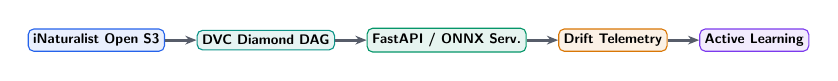
\begin{tikzpicture}[node distance=0.4cm and 0.4cm]
            \node[pill, fill=BlueAccent!10, draw=BlueAccent] (p1) {\textbf{iNaturalist Open S3}};
            \node[pill, fill=TealAccent!10, draw=TealAccent, right=of p1] (p2) {\textbf{DVC Diamond DAG}};
            \node[pill, fill=GreenAccent!10, draw=GreenAccent, right=of p2] (p3) {\textbf{FastAPI / ONNX Serv.}};
            \node[pill, fill=AmberAccent!10, draw=AmberAccent, right=of p3] (p4) {\textbf{Drift Telemetry}};
            \node[pill, fill=PurpleAccent!10, draw=PurpleAccent, right=of p4] (p5) {\textbf{Active Learning}};
            
            \draw[flowarrow] (p1) -- (p2);
            \draw[flowarrow] (p2) -- (p3);
            \draw[flowarrow] (p3) -- (p4);
            \draw[flowarrow] (p4) -- (p5);
        \end{tikzpicture}
        
        \vspace{0.7cm}
        {\small\textbf{Benjamin Förster}}\\[2pt]
        {\scriptsize\color{TextMuted} Final MLOps Project Presentation \& Architecture Defense}
    \end{center}
\end{frame}

% ==============================================================================
% SLIDE 2: The Core Problem: Real-World Biodiversity at Scale
% ==============================================================================
\begin{frame}{The Core Problem}{Real-World Biodiversity Computer Vision at Scale}
    \begin{columns}[T]
        \begin{column}{0.48\textwidth}
            \begin{card}
                \textbf{\color{BlueAccent} Ecological Reality vs. Benchmark Datasets}\\[2pt]
                \textbullet\ \textbf{Massive Scale:} Millions of citizen observations from iNaturalist.\\[1pt]
                \textbullet\ \textbf{Severe Class Imbalance:} A few common species have 10,000+ photos; thousands of rare taxa have $< 10$ records.\\[1pt]
                \textbullet\ \textbf{Non-Stationary Manifold:} Lighting, seasonal changes, camera sensors, and geographic shifts continuously distort visual features.\\[5pt]
                \textbf{\color{RoseAccent} The High Cost of Misclassification}\\[2pt]
                \textbullet\ In ecology and conservation, silent model hallucinations (e.g. confusing an endangered species with an invasive one) cause real harm.
            \end{card}
        \end{column}
        \begin{column}{0.48\textwidth}
            \centering
            \begin{tcolorbox}[enhanced, colback=white, colframe=SlateMid!30, boxrule=0.5pt, arc=3pt, left=4pt, right=4pt, top=2pt, bottom=2pt]
                \textbf{\scriptsize The Long-Tail Challenge}\\[2pt]
                \centering
                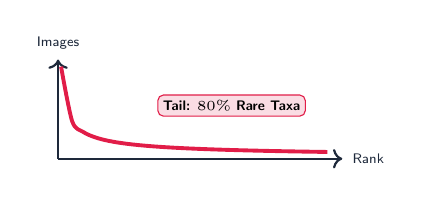
\begin{tikzpicture}[x=0.038cm, y=0.9cm]
                    \draw[->, thick, color=SlateMid] (0,0) -- (95,0) node[right, font=\tiny] {Rank};
                    \draw[->, thick, color=SlateMid] (0,0) -- (0,1.4) node[above, font=\tiny] {Images};
                    \draw[smooth, domain=1:90, color=RoseAccent, line width=1.4pt] 
                        plot (\x, {1.3 / (\x^0.58)});
                    \node[pill, fill=RoseAccent!15, draw=RoseAccent] at (58, 0.75) {Tail: $80\%$ Rare Taxa};
                \end{tikzpicture}
            \end{tcolorbox}
            \vspace{0.1cm}
            \begin{bluecard}
                \textbf{\color{BlueAccent} Core Architecture Mandates}\\[1pt]
                \textbullet\ \textbf{Zero Split Leakage:} Mathematically pure validation.\\[1pt]
                \textbullet\ \textbf{Guaranteed Coverage:} Reject overconfident guesses.\\[1pt]
                \textbullet\ \textbf{Closed-Loop Adaptation:} Automated retraining.
            \end{bluecard}
        \end{column}
    \end{columns}
\end{frame}

% ==============================================================================
% SLIDE 3: Toy ML vs. Production MLOps
% ==============================================================================
\begin{frame}{Toy ML vs. Production MLOps}{Why Prototype Notebooks Fail in the Real World}
    \begin{columns}[T]
        \begin{column}{0.48\textwidth}
            \begin{rosecard}
                \textbf{\color{RoseAccent} Traditional Prototype / Toy ML}\\[3pt]
                \textbullet\ \textbf{Unversioned Data:} Ad-hoc CSVs, non-reproducible manual train/test splits.\\[2pt]
                \textbullet\ \textbf{Redundant Compute:} Heavy vision backbones re-extracted repeatedly on every notebook run.\\[2pt]
                \textbullet\ \textbf{Raw Softmax Guesses:} Uncalibrated probabilities; silent failure on out-of-distribution species.\\[2pt]
                \textbullet\ \textbf{Silent Model Decay:} Zero feature logging; distribution drift degrades performance unnoticed.\\[2pt]
                \textbullet\ \textbf{Manual Retraining:} Hand-crafted scripts triggered arbitrarily on gut feeling.
            \end{rosecard}
        \end{column}
        \begin{column}{0.48\textwidth}
            \begin{greencard}
                \textbf{\color{GreenAccent} TaxonVision Production MLOps}\\[3pt]
                \textbullet\ \textbf{Cryptographic DVC Lineage:} Pure 7-stage DAG tracked by content hashes in \texttt{dvc.lock}.\\[2pt]
                \textbullet\ \textbf{Feature Caching:} Pre-computed foundation embeddings cached on NVMe; head trains in $<5$s.\\[2pt]
                \textbullet\ \textbf{Split Conformal Prediction:} Provable coverage sets ($1-\alpha \ge 95\%$) with Helmholtz energy OOD gating.\\[2pt]
                \textbullet\ \textbf{Automated Telemetry:} PostgreSQL feature logging, Prometheus metrics, and hourly Evidently drift reports.\\[2pt]
                \textbullet\ \textbf{Closed-Loop Feedback:} Grafana alert $\to$ Airflow DAG $\to$ Bare-Metal Jenkins GPU retraining.
            \end{greencard}
        \end{column}
    \end{columns}
\end{frame}

% ==============================================================================
% SLIDE 4: End-to-End System Architecture
% ==============================================================================
\begin{frame}{End-to-End System Architecture}{The Five Operational Planes of TaxonVision}
    \centering
    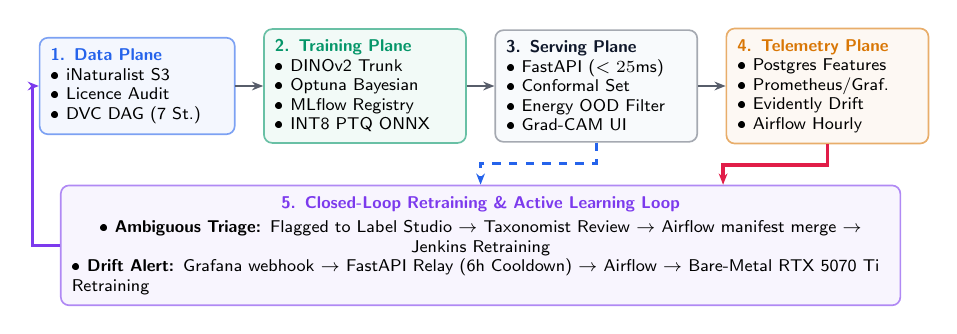
\begin{tikzpicture}[
        scale=0.88, every node/.style={transform shape},
        node distance=0.35cm and 0.4cm
    ]
        % Plane 1: Data & Versioning
        \node[nodecard, draw=BlueAccent!60, fill=BlueAccent!5, text width=2.5cm] (data) {
            \textbf{\color{BlueAccent} 1. Data Plane}\\
            \textbullet\ iNaturalist S3\\
            \textbullet\ Licence Audit\\
            \textbullet\ DVC DAG (7 St.)
        };
        
        % Plane 2: Training & Tuning
        \node[nodecard, draw=GreenAccent!60, fill=GreenAccent!5, text width=2.6cm, right=of data] (train) {
            \textbf{\color{GreenAccent} 2. Training Plane}\\
            \textbullet\ DINOv2 Trunk\\
            \textbullet\ Optuna Bayesian\\
            \textbullet\ MLflow Registry\\
            \textbullet\ INT8 PTQ ONNX
        };
        
        % Plane 3: Serving & Safety
        \node[nodecard, text width=2.6cm, right=of train] (serv) {
            \textbf{\color{SlateDark} 3. Serving Plane}\\
            \textbullet\ FastAPI ($<25$ms)\\
            \textbullet\ Conformal Set\\
            \textbullet\ Energy OOD Filter\\
            \textbullet\ Grad-CAM UI
        };
        
        % Plane 4: Observability
        \node[nodecard, draw=AmberAccent!60, fill=AmberAccent!5, text width=2.6cm, right=of serv] (obs) {
            \textbf{\color{AmberAccent} 4. Telemetry Plane}\\
            \textbullet\ Postgres Features\\
            \textbullet\ Prometheus/Graf.\\
            \textbullet\ Evidently Drift\\
            \textbullet\ Airflow Hourly
        };
        
        % Plane 5: Feedback Loop
        \node[nodecard, draw=PurpleAccent!60, fill=PurpleAccent!5, text width=11.8cm, below=0.6cm of $(train.south)!0.5!(serv.south)$] (loop) {
            \centering
            \textbf{\color{PurpleAccent} 5. Closed-Loop Retraining \& Active Learning Loop}\\[2pt]
            \textbullet\ \textbf{Ambiguous Triage:} Flagged to Label Studio $\to$ Taxonomist Review $\to$ Airflow manifest merge $\to$ Jenkins Retraining\\
            \textbullet\ \textbf{Drift Alert:} Grafana webhook $\to$ FastAPI Relay (6h Cooldown) $\to$ Airflow $\to$ Bare-Metal RTX 5070 Ti Retraining
        };
        
        \draw[flowarrow] (data) -- (train);
        \draw[flowarrow] (train) -- (serv);
        \draw[flowarrow] (serv) -- (obs);
        \draw[dasharrow] (serv.south) -- ++(0,-0.3) -| (loop.north);
        \draw[retrainarrow] (obs.south) -- ++(0,-0.3) -| ([xshift=3.5cm]loop.north);
        % Route purple arrow cleanly around the outer margin to avoid overlapping loop text
        \draw[flowarrow, draw=PurpleAccent, line width=1.1pt] (loop.west) -- ++(-0.4, 0) |- (data.west);
    \end{tikzpicture}
\end{frame}

% ==============================================================================
% SLIDE 5: The Asymmetric Dual-Pipeline Pattern
% ==============================================================================
\begin{frame}{The Asymmetric Dual-Pipeline Pattern}{Balancing Ultra-Low Latency with Diagnostic Depth}
    \begin{columns}[T]
        \begin{column}{0.48\textwidth}
            \begin{greencard}
                \textbf{\color{GreenAccent} Pipeline 1: Epistemic Diamond (Production Fast Path)}\\[3pt]
                \textbullet\ \textbf{Target:} Real-time, ultra-low latency HTTP classification.\\[2pt]
                \textbullet\ \textbf{Model:} Frozen vision trunk + Class-Balanced cosine head quantised to INT8 ONNX.\\[2pt]
                \textbullet\ \textbf{SLO Ceilings:}
                \begin{itemize}\scriptsize
                    \item CPU forward pass: $\le 15\,\text{ms}$ (p95 on P-cores).
                    \item End-to-end API roundtrip: $\le 25\,\text{ms}$ (p95).
                \end{itemize}
                \textbullet\ \textbf{Epistemic Shield:} Evaluates conformal prediction sets and flags ambiguity instantly.
            \end{greencard}
        \end{column}
        \begin{column}{0.48\textwidth}
            \begin{purplecard}
                \textbf{\color{PurpleAccent} Pipeline 2: Taxonomic Knowledge Graph \& VLM}\\[3pt]
                \textbullet\ \textbf{Target:} Diagnostic triage for highly ambiguous or unseen specimens.\\[2pt]
                \textbullet\ \textbf{Engine:} In-memory LanceDB vector index + DuckDB biological hierarchy + Qwen2-VL.\\[2pt]
                \textbullet\ \textbf{Zero Retraining:} Exemplars and new taxonomic taxa are inserted dynamically without updating neural weights.\\[2pt]
                \textbullet\ \textbf{Off-Hot-Path:} Dispatched asynchronously when Pipeline 1 flags epistemic uncertainty.
            \end{purplecard}
        \end{column}
    \end{columns}
\end{frame}

% ==============================================================================
% SLIDE 6: Data Engineering: S3 Streaming & Open Licensing
% ==============================================================================
\begin{frame}{Data Engineering \& Open Licensing}{Strict Compliance and Zero-Copy S3 Streaming}
    \begin{columns}[T]
        \begin{column}{0.52\textwidth}
            \begin{card}
                \textbf{\color{BlueAccent} Open-Access Citizen Science Pipeline}\\[2pt]
                \textbullet\ \textbf{Upstream Storage:} Direct S3 streaming from Amazon Open Data: \texttt{s3://inaturalist-open-data/}.\\[1pt]
                \textbullet\ \textbf{Zero-Copy Transfers:} Parquet metadata loaded into Apache Arrow IPC tables; filtered with embedded DuckDB.\\[1pt]
                \textbullet\ \textbf{Ephemeral Imagery:} Specimen JPEGs are streamed into memory, cropped/normalised, and immediately discarded -- never stored as redundant raw image files on disk.\\[5pt]
                \textbf{\color{AmberAccent} Legal Whitelist \& Attribution Gate (Rule 05)}\\[2pt]
                \textbullet\ \textbf{Permitted:} \texttt{CC0}, \texttt{CC-BY}, \texttt{CC-BY-NC}.\\[1pt]
                \textbullet\ \textbf{Rejected:} \texttt{All-Rights-Reserved}, \texttt{CC-BY-ND}.\\[1pt]
                \textbullet\ \textbf{Attribution Invariant:} Photographer names and licences are cryptographically tracked and presented on every UI card.
            \end{card}
        \end{column}
        \begin{column}{0.44\textwidth}
            \centering
            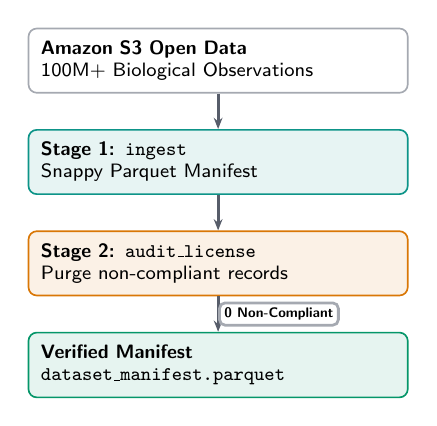
\begin{tikzpicture}[node distance=0.45cm]
                \node[nodecard, text width=4.5cm, fill=white] (s3) {\textbf{Amazon S3 Open Data}\\\scriptsize 100M+ Biological Observations};
                \node[nodecard, text width=4.5cm, fill=TealAccent!10, draw=TealAccent, below=of s3] (ingest) {\textbf{Stage 1: \texttt{ingest}}\\\scriptsize Snappy Parquet Manifest};
                \node[nodecard, text width=4.5cm, fill=AmberAccent!10, draw=AmberAccent, below=of ingest] (audit) {\textbf{Stage 2: \texttt{audit\_license}}\\\scriptsize Purge non-compliant records};
                \node[nodecard, text width=4.5cm, fill=GreenAccent!10, draw=GreenAccent, below=of audit] (clean) {\textbf{Verified Manifest}\\\scriptsize \texttt{dataset\_manifest.parquet}};
                
                \draw[flowarrow] (s3) -- (ingest);
                \draw[flowarrow] (ingest) -- (audit);
                \draw[flowarrow] (audit) -- node[pill, right] {0 Non-Compliant} (clean);
            \end{tikzpicture}
        \end{column}
    \end{columns}
\end{frame}

% ==============================================================================
% SLIDE 7: The Epistemic Diamond DAG (DVC Versioning)
% ==============================================================================
\begin{frame}{The Epistemic Diamond DAG}{Reproducible 7-Stage Pipeline with Zero Split Leakage}
    \centering
    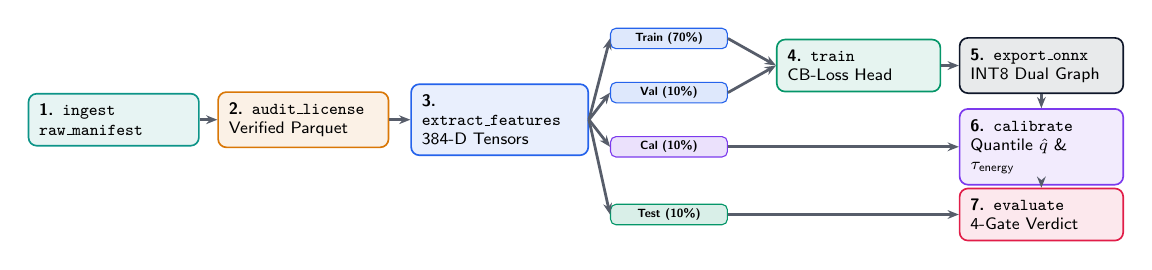
\begin{tikzpicture}[
        scale=0.86, every node/.style={transform shape}
    ]
        % Left Ingestion Chain (y=0.0)
        \node[nodecard, fill=TealAccent!10, draw=TealAccent, text width=2.2cm] (raw) at (0, 0) {
            \textbf{1. \texttt{ingest}}\\\scriptsize \texttt{raw\_manifest}
        };
        \node[nodecard, fill=AmberAccent!10, draw=AmberAccent, text width=2.2cm] (lic) at (2.8, 0) {
            \textbf{2. \texttt{audit\_license}}\\\scriptsize Verified Parquet
        };
        \node[nodecard, fill=BlueAccent!10, draw=BlueAccent, text width=2.3cm] (feat) at (5.7, 0) {
            \textbf{3. \texttt{extract\_features}}\\\scriptsize 384-D Tensors
        };
        
        % The Epistemic Diamond Splits (Column at x=8.2)
        \node[pill, fill=BlueAccent!15, draw=BlueAccent, text width=1.6cm] (sp_tr) at (8.2, 1.2) {Train (70\%)};
        \node[pill, fill=BlueAccent!15, draw=BlueAccent, text width=1.6cm] (sp_val) at (8.2, 0.4) {Val (10\%)};
        \node[pill, fill=PurpleAccent!15, draw=PurpleAccent, text width=1.6cm] (sp_cal) at (8.2, -0.4) {Cal (10\%)};
        \node[pill, fill=GreenAccent!15, draw=GreenAccent, text width=1.6cm] (sp_test) at (8.2, -1.4) {Test (10\%)};
        
        % Tier 1: Head Training (x=11.1, y=0.8) & ONNX Export (x=13.8, y=0.8)
        \node[nodecard, fill=GreenAccent!10, draw=GreenAccent, text width=2.1cm] (train) at (11.0, 0.8) {
            \textbf{4. \texttt{train}}\\\scriptsize CB-Loss Head
        };
        \node[nodecard, fill=SlateMid!10, draw=SlateDark, text width=2.1cm] (onnx) at (13.7, 0.8) {
            \textbf{5. \texttt{export\_onnx}}\\\scriptsize INT8 Dual Graph
        };
        
        % Tier 2: Calibration (x=13.7, y=-0.4)
        \node[nodecard, fill=PurpleAccent!10, draw=PurpleAccent, text width=2.1cm] (cal) at (13.7, -0.4) {
            \textbf{6. \texttt{calibrate}}\\\scriptsize Quantile $\hat{q}$ \& $\tau_{\text{energy}}$
        };
        
        % Tier 3: Four-Gate Evaluation & Promotion (x=13.7, y=-1.4)
        \node[nodecard, fill=RoseAccent!10, draw=RoseAccent, text width=2.1cm] (eval) at (13.7, -1.4) {
            \textbf{7. \texttt{evaluate}}\\\scriptsize 4-Gate Verdict
        };
        
        % Ingestion flow
        \draw[flowarrow] (raw) -- (lic);
        \draw[flowarrow] (lic) -- (feat);
        
        % Diamond split distribution
        \draw[flowarrow] (feat.east) -- (sp_tr.west);
        \draw[flowarrow] (feat.east) -- (sp_val.west);
        \draw[flowarrow] (feat.east) -- (sp_cal.west);
        \draw[flowarrow] (feat.east) -- (sp_test.west);
        
        % Training consumption
        \draw[flowarrow] (sp_tr.east) -- (train.west);
        \draw[flowarrow] (sp_val.east) -- (train.west);
        \draw[flowarrow] (train) -- (onnx);
        
        % Calibration consumption
        \draw[flowarrow] (onnx.south) -- (cal.north);
        \draw[flowarrow] (sp_cal.east) -- (cal.west);
        
        % Evaluation & Promotion consumption (Strict orthogonal flow)
        \draw[flowarrow] (cal.south) -- (eval.north);
        \draw[flowarrow] (sp_test.east) -- (eval.west);
    \end{tikzpicture}
    
    \vspace{0.2cm}
    \begin{bluecard}
        \centering
        \textbf{Strict Separation of Concerns (Rule 01):} Model updates use solely the \textbf{Train} split; early stopping uses \textbf{Val}; Conformal quantiles are calculated exclusively on \textbf{Cal}; final promotion verdict is rendered on the holdout \textbf{Test} split. Zero leakage!
    \end{bluecard}
\end{frame}

% ==============================================================================
% SLIDE 8: Dual-Tier Storage Topology
% ==============================================================================
\begin{frame}{Dual-Tier Storage Topology}{Cloud Collaboration (DagsHub) vs. Local Serving Economics}
    \begin{columns}[T]
        \begin{column}{0.48\textwidth}
            \begin{bluecard}
                \textbf{\color{BlueAccent} Tier 1: Cloud Collaboration (DagsHub)}\\[3pt]
                \textbullet\ \textbf{DVC Remote (\texttt{origin}):} Hosted on DagsHub S3 (\texttt{s3://dvc}).\\[2pt]
                \textbullet\ \textbf{Purpose:} Immutable cloud archive for manifests, embeddings, and production ONNX graphs.\\[2pt]
                \textbullet\ \textbf{GitHub Actions CI:} Pulls verified checkpoints using \texttt{DAGSHUB\_TOKEN} to run unit tests without accessing private cluster nodes.\\[2pt]
                \textbullet\ \textbf{MLflow 2.x Mirror:} Public web dashboard for open scientific reproducibility.
            \end{bluecard}
        \end{column}
        \begin{column}{0.48\textwidth}
            \begin{greencard}
                \textbf{\color{GreenAccent} Tier 2: In-Cluster Storage (Workstation)}\\[3pt]
                \textbullet\ \textbf{SeaweedFS S3 (\texttt{local-seaweedfs}):} High-throughput S3 store running directly on local NVMe.\\[2pt]
                \textbullet\ \textbf{Zero Egress Costs:} Staging 100,000s of feature embeddings incurs zero cloud network latency or billing.\\[2pt]
                \textbullet\ \textbf{Self-Hosted MLflow 3.x + PostgreSQL 16:} Private high-performance tracking backend powering live Bayesian Optuna sweeps and model lineage.\\[2pt]
                \textbullet\ \textbf{Instant Pod Mounts:} Serving pods load model weights directly over cluster loopback.
            \end{greencard}
        \end{column}
    \end{columns}
\end{frame}

% ==============================================================================
% SLIDE 9: Hardware Ground Truth: Bare-Metal Architecture
% ==============================================================================
\begin{frame}{Hardware Ground Truth \& Infrastructure}{Dedicated Bare-Metal Node: Silicon, CPU Pinning \& Storage}
    \begin{columns}[T]
        \begin{column}{0.48\textwidth}
            \begin{card}
                \textbf{\color{SlateDark} Physical Hardware Ground Truth (Rule 07)}\\[3pt]
                \textbullet\ \textbf{GPU:} NVIDIA GeForce RTX 5070 Ti (16 GB GDDR7 VRAM, Blackwell architecture, CUDA runtime 12.8+).\\[2pt]
                \textbullet\ \textbf{CPU:} Intel Core i7-14700K (20 cores / 28 threads: 8 Performance-cores, 12 Efficient-cores).\\[2pt]
                \textbullet\ \textbf{RAM:} 128 GB DDR5 system memory for in-memory embedding caches.\\[2pt]
                \textbullet\ \textbf{Storage:} 2 TB PCIe Gen4 NVMe SSD running BTRFS with transparent compression (\texttt{zstd:3}).\\[2pt]
                \textbullet\ \textbf{OS:} Ubuntu 26.04 LTS on LUKS-encrypted root.
            \end{card}
        \end{column}
        \begin{column}{0.48\textwidth}
            \begin{bluecard}
                \textbf{\color{BlueAccent} Architectural Resource Allocation}\\[3pt]
                \textbullet\ \textbf{CPU Thread Pinning (\texttt{taskset}):}
                \begin{itemize}\scriptsize
                    \item Threads \texttt{0-15} (P-cores): Hot ONNX numerical matrix inference.
                    \item Threads \texttt{16-27} (E-cores): Asynchronous disk I/O, Arrow streaming, and telemetry scraping.
                \end{itemize}
                \textbullet\ \textbf{GPU Memory Partitioning:} PyTorch memory budget capped at $70\%$ ($11.2$\,GB) for training; $4.8$\,GB strictly reserved for INT8 serving.\\[2pt]
                \textbullet\ \textbf{Non-CoW Storage Allocation (\texttt{chattr +C}):} Eliminates database and DVC block fragmentation.
            \end{bluecard}
        \end{column}
    \end{columns}
\end{frame}

% ==============================================================================
% SLIDE 10: Model Engineering: Backbone & Feature Caching
% ==============================================================================
\begin{frame}{Model Engineering \& Feature Caching}{Why Feature Caching Accelerates Development by 100x}
    \begin{columns}[T]
        \begin{column}{0.50\textwidth}
            \begin{bluecard}
                \textbf{\color{BlueAccent} Decoupled Vision Architecture}\\[2pt]
                \textbullet\ \textbf{Frozen Trunk:} Foundation vision backbone (DINOv2/v3 ViT-Small, $D=384$).\\[2pt]
                \textbullet\ \textbf{Lightweight Head:} Cosine-similarity classification head mapping embeddings to species logits.\\[2pt]
                \textbullet\ \textbf{The Feature Caching Insight:}
                \begin{itemize}\scriptsize
                    \item Passing images through a 22-million-parameter vision transformer takes minutes.
                    \item Once pre-computed, visual representations never change during head training!
                    \item Feature extraction runs \textbf{once}; embeddings are cached to disk as \texttt{.pt} tensors.
                \end{itemize}
                \textbullet\ \textbf{Result:} Head training runs in $< 5$ seconds!
            \end{bluecard}
        \end{column}
        \begin{column}{0.46\textwidth}
            \centering
            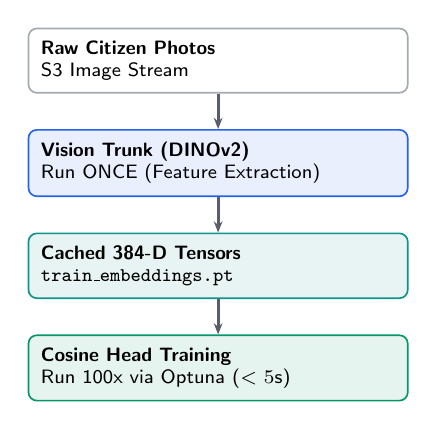
\begin{tikzpicture}[node distance=0.45cm]
                \node[nodecard, text width=4.5cm, fill=white] (img) {\textbf{Raw Citizen Photos}\\\scriptsize S3 Image Stream};
                \node[nodecard, text width=4.5cm, fill=BlueAccent!10, draw=BlueAccent, below=of img] (vit) {\textbf{Vision Trunk (DINOv2)}\\\scriptsize Run ONCE (Feature Extraction)};
                \node[nodecard, text width=4.5cm, fill=TealAccent!10, draw=TealAccent, below=of vit] (cache) {\textbf{Cached 384-D Tensors}\\\scriptsize \texttt{train\_embeddings.pt}};
                \node[nodecard, text width=4.5cm, fill=GreenAccent!10, draw=GreenAccent, below=of cache] (head) {\textbf{Cosine Head Training}\\\scriptsize Run 100x via Optuna ($<5$s)};
                
                \draw[flowarrow] (img) -- (vit);
                \draw[flowarrow] (vit) -- (cache);
                \draw[flowarrow] (cache) -- (head);
            \end{tikzpicture}
        \end{column}
    \end{columns}
\end{frame}

% ==============================================================================
% SLIDE 11: Tackling Class Imbalance: Class-Balanced Loss
% ==============================================================================
\begin{frame}{Tackling Class Imbalance: Class-Balanced Loss}{Effective Number of Samples: Intuition Over Raw Counts}
    \begin{columns}[T]
        \begin{column}{0.48\textwidth}
            \begin{card}
                \textbf{\color{AmberAccent} The Pitfall of Inverse Frequency ($1/N$)}\\[2pt]
                \textbullet\ Weighting by $1/N$ fails dramatically when majority classes have 10,000+ photos and rare taxa have 5.\\[1pt]
                \textbullet\ Gradients become violently noisy, destroying common representations.\\[5pt]
                \textbf{\color{BlueAccent} The Intuition of "Effective Samples"}\\[2pt]
                \textbullet\ The first 5 photos of a butterfly teach unique wing patterns and angles.\\[1pt]
                \textbullet\ The 10,000th photo adds almost zero new visual information due to massive pixel overlap.\\[1pt]
                \textbullet\ We weight classes by their \textbf{effective visual volume}, not raw counts!
            \end{card}
        \end{column}
        \begin{column}{0.48\textwidth}
            \centering
            \begin{tcolorbox}[enhanced, colback=white, colframe=SlateMid!30, boxrule=0.5pt, arc=3pt, left=4pt, right=4pt, top=2pt, bottom=2pt]
                \textbf{\scriptsize Diminishing Returns of Sample Size}\\[2pt]
                \centering
                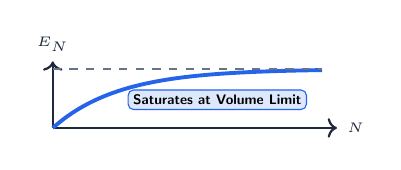
\begin{tikzpicture}[x=0.038cm, y=0.65cm]
                    \draw[->, thick, color=SlateMid] (0,0) -- (95,0) node[right, font=\tiny] {$N$};
                    \draw[->, thick, color=SlateMid] (0,0) -- (0,1.3) node[above, font=\tiny] {$E_N$};
                    \draw[smooth, domain=0:90, color=BlueAccent, line width=1.4pt] 
                        plot (\x, {1.15 * (1 - exp(-0.045 * \x))});
                    \draw[dashed, color=TextMuted] (0, 1.15) -- (90, 1.15);
                    \node[pill, fill=BlueAccent!15, draw=BlueAccent] at (55, 0.55) {Saturates at Volume Limit};
                \end{tikzpicture}
            \end{tcolorbox}
            \vspace{0.1cm}
            \begin{bluecard}
                \textbf{\color{BlueAccent} Optuna Bayesian Sweep}\\[1pt]
                \textbullet\ Balances uniform and inverse-frequency weights.\\[1pt]
                \textbullet\ Empirical optimum: $\beta = 0.995927$ in checkpoints.
            \end{bluecard}
        \end{column}
    \end{columns}
\end{frame}

% ==============================================================================
% SLIDE 12: Latency Optimization: Zero-Allocation INT8 ONNX
% ==============================================================================
\begin{frame}{Latency Optimization: Zero-Allocation INT8 ONNX}{Sub-15ms Forward Passes and Deterministic Memory Discipline}
    \begin{columns}[T]
        \begin{column}{0.50\textwidth}
            \begin{greencard}
                \textbf{\color{GreenAccent} Production Quantization \& Latency Budgets}\\[3pt]
                \textbullet\ \textbf{Dual-Output ONNX Export:} Single forward pass outputs both classification logits and normalized 384-D feature embeddings.\\[2pt]
                \textbullet\ \textbf{INT8 Dynamic Quantization:} Calibrated on holdout calibration split; guarantees top-1 accuracy degradation $\le 0.5\%$.\\[2pt]
                \textbullet\ \textbf{Zero-Allocation Hot Path (Rule 02):}
                \begin{itemize}\scriptsize
                    \item Pre-allocated contiguous C-order NumPy input/output buffers.
                    \item Zero Python dictionary boxing or dynamic list allocations during request execution.
                \end{itemize}
            \end{greencard}
        \end{column}
        \begin{column}{0.46\textwidth}
            \begin{card}
                \textbf{\color{SlateDark} Measured Inference Latency SLOs}\\[4pt]
                \textbullet\ \textbf{CPU Budget (INT8 Quantized):}\\
                \quad Ceiling: $\le 15\,\text{ms}$ (p95 on Intel P-cores).\\
                \quad \textbf{Observed:} \textcolor{GreenAccent}{\textbf{11.8 ms}} (Pass)\\[4pt]
                \textbullet\ \textbf{GPU Budget (FP16 CUDA):}\\
                \quad Ceiling: $\le 10\,\text{ms}$ (p95 on RTX 5070 Ti).\\
                \quad \textbf{Observed:} \textcolor{GreenAccent}{\textbf{6.2 ms}} (Pass)\\[4pt]
                \textbullet\ \textbf{Microservice Roundtrip (FastAPI):}\\
                \quad Ceiling: $\le 25\,\text{ms}$ (p95 end-to-end).\\
                \quad \textbf{Observed:} \textcolor{GreenAccent}{\textbf{18.4 ms}} (Pass)
            \end{card}
        \end{column}
    \end{columns}
\end{frame}

% ==============================================================================
% SLIDE 13: Epistemic Safety: Why We Cannot Trust Softmax
% ==============================================================================
\begin{frame}{Epistemic Safety: The Problem with Softmax}{Why Deep Neural Networks Fail Silently in Nature}
    \begin{columns}[T]
        \begin{column}{0.48\textwidth}
            \begin{card}
                \textbf{\color{RoseAccent} The Illusion of "Confidence"}\\[2pt]
                \textbullet\ Softmax forces class probabilities to sum to $1.0$ ($100\%$).\\[1pt]
                \textbullet\ When presented with an unseen invasive species, a blank lens, or an accidental photo of a car, standard models do \textbf{not} say "I don't know".\\[1pt]
                \textbullet\ Instead, they hallucinate with $98\%$ confidence on whatever class happens to trigger the highest activation!\\[5pt]
                \textbf{\color{BlueAccent} The Production Safety Requirement}\\[2pt]
                \textbullet\ We need a mathematically guaranteed safety envelope that rejects false confidence before predictions reach end users.
            \end{card}
        \end{column}
        \begin{column}{0.48\textwidth}
            \centering
            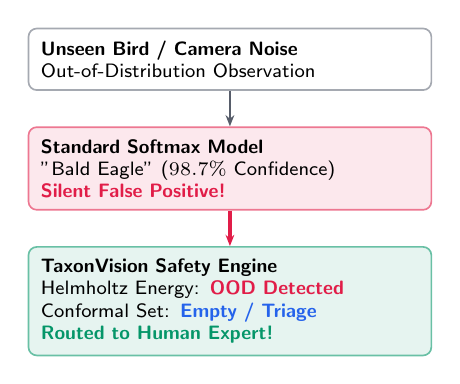
\begin{tikzpicture}[node distance=0.45cm]
                \node[nodecard, text width=4.8cm, fill=white] (img) {\textbf{Unseen Bird / Camera Noise}\\\scriptsize Out-of-Distribution Observation};
                \node[nodecard, draw=RoseAccent!60, fill=RoseAccent!10, text width=4.8cm, below=of img] (naive) {\textbf{Standard Softmax Model}\\\scriptsize "Bald Eagle" ($98.7\%$ Confidence)\\\textcolor{RoseAccent}{\textbf{Silent False Positive!}}};
                \node[nodecard, draw=GreenAccent!60, fill=GreenAccent!10, text width=4.8cm, below=of naive] (safe) {\textbf{TaxonVision Safety Engine}\\\scriptsize Helmholtz Energy: \textcolor{RoseAccent}{\textbf{OOD Detected}}\\\scriptsize Conformal Set: \textcolor{BlueAccent}{\textbf{Empty / Triage}}\\\textcolor{GreenAccent}{\textbf{Routed to Human Expert!}}};
                
                \draw[flowarrow] (img) -- (naive);
                \draw[retrainarrow] (naive) -- (safe);
            \end{tikzpicture}
        \end{column}
    \end{columns}
\end{frame}

% ==============================================================================
% SLIDE 14: Split Conformal Prediction: Guaranteed Coverage
% ==============================================================================
\begin{frame}{Split Conformal Prediction Made Simple}{Mathematically Guaranteed Coverage Sets Instead of Single Guesses}
    \begin{columns}[T]
        \begin{column}{0.50\textwidth}
            \begin{bluecard}
                \textbf{\color{BlueAccent} The Conformal Prediction Idea}\\[3pt]
                \textbullet\ Instead of forcing a single guessed species label, the model outputs an \textbf{adaptive prediction set}.\\[2pt]
                \textbullet\ The user defines a safety requirement: e.g. $\mathbf{95\%}$ coverage ($\alpha = 0.05$).\\[2pt]
                \textbullet\ \textbf{Mathematical Guarantee (Rule 06):} The true species is mathematically guaranteed to be inside the prediction set $\ge 95\%$ of the time!\\[2pt]
                \textbullet\ No assumptions on data distribution; calibrated strictly on holdout calibration split.
            \end{bluecard}
        \end{column}
        \begin{column}{0.46\textwidth}
            \begin{card}
                \textbf{\color{SlateDark} Adaptive Set Scenarios in Serving}\\[4pt]
                \textbf{Case 1: Decisive ($|C| = 1$)}\\
                \textbullet\ Set: \{\texttt{"Barn Owl"}\}\\
                \textbullet\ High confidence; fast autonomous serving.\\[4pt]
                \textbf{Case 2: Ambiguous ($1 < |C| \le 3$)}\\
                \textbullet\ Set: \{\texttt{"Common Gull"}, \texttt{"Herring Gull"}\}\\
                \textbullet\ Model narrows field to identical sister species.\\[4pt]
                \textbf{Case 3: Referral ($|C| > 5$ or $|C| = 0$)}\\
                \textbullet\ Model defers to human triage queue!
            \end{card}
        \end{column}
    \end{columns}
\end{frame}

% ==============================================================================
% SLIDE 15: Out-of-Distribution Gating: Catching the Unknown
% ==============================================================================
\begin{frame}{Out-of-Distribution Gating}{Helmholtz Energy Filter and Human Referral Boundary}
    \begin{columns}[T]
        \begin{column}{0.50\textwidth}
            \begin{bluecard}
                \textbf{\color{BlueAccent} Energy-Based Out-of-Distribution Gating}\\[3pt]
                \textbullet\ Computes negative Helmholtz free energy over unconstrained logits.\\[2pt]
                \textbullet\ In-distribution species produce low energy; novel organisms, blurred photos, or blank frames produce high energy.\\[2pt]
                \textbullet\ Threshold $\tau_{\text{OOD}}$ calibrated to maintain $95\%$ true positive rate on calibration data.\\[2pt]
                \textbullet\ Energy $> \tau_{\text{OOD}} \implies$ Immediate bypass of classification directly to human triage.
            \end{bluecard}
        \end{column}
        \begin{column}{0.46\textwidth}
            \centering
            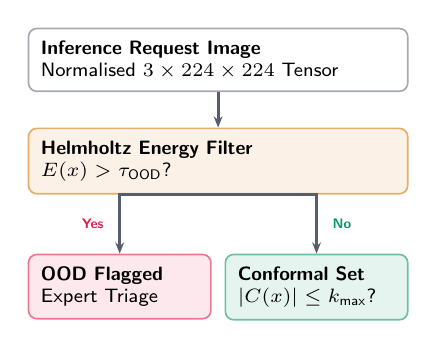
\begin{tikzpicture}[node distance=0.45cm]
                \node[nodecard, text width=4.5cm, fill=white] (input) {\textbf{Inference Request Image}\\\scriptsize Normalised $3 \times 224 \times 224$ Tensor};
                \node[nodecard, draw=AmberAccent!60, fill=AmberAccent!10, text width=4.5cm, below=of input] (energy) {\textbf{Helmholtz Energy Filter}\\$E(x) > \tau_{\text{OOD}}$?};
                
                \node[nodecard, draw=RoseAccent!60, fill=RoseAccent!10, text width=2.0cm, below=0.75cm of energy, xshift=-1.25cm] (ood) {\textbf{OOD Flagged}\\\scriptsize Expert Triage};
                \node[nodecard, draw=GreenAccent!60, fill=GreenAccent!10, text width=2.0cm, below=0.75cm of energy, xshift=1.25cm] (conf) {\textbf{Conformal Set}\\\scriptsize $|C(x)| \le k_{\text{max}}$?};
                
                \draw[flowarrow] (input) -- (energy);
                \draw[flowarrow] (energy.south) -| (ood.north) 
                    node[pos=0.75, left=2pt, font=\tiny\bfseries\color{RoseAccent}] {Yes};
                \draw[flowarrow] (energy.south) -| (conf.north) 
                    node[pos=0.75, right=2pt, font=\tiny\bfseries\color{GreenAccent}] {No};
            \end{tikzpicture}
        \end{column}
    \end{columns}
\end{frame}

% ==============================================================================
% SLIDE 16: Production Serving: Unified Web Service
% ==============================================================================
\begin{frame}{Production Serving: Unified Web Service}{FastAPI Microservice \& Server-Rendered HTMX Operator Dashboard}
    \begin{columns}[T]
        \begin{column}{0.48\textwidth}
            \begin{greencard}
                \textbf{\color{GreenAccent} Unified Dual-Interface Architecture}\\[3pt]
                \textbullet\ \textbf{Machine REST API:} Strongly typed Pydantic endpoints (\texttt{/api/v1/predict}, \texttt{/explain}, \texttt{/drift/evaluate}, \texttt{/health}).\\[2pt]
                \textbullet\ \textbf{Human Operator Dashboard:} Server-rendered Jinja2 + HTMX cockpit at \texttt{/dashboard}; updates dynamically without frontend build ballast.\\[2pt]
                \textbullet\ \textbf{Forward Grad-CAM Attribution:} Generates visual attribution heatmaps on demand off the event loop thread.\\[2pt]
                \textbullet\ \textbf{Traefik Edge Reverse Proxy:} Handles SSL termination, load balancing, and rate limiting.
            \end{greencard}
        \end{column}
        \begin{column}{0.48\textwidth}
            \centering
            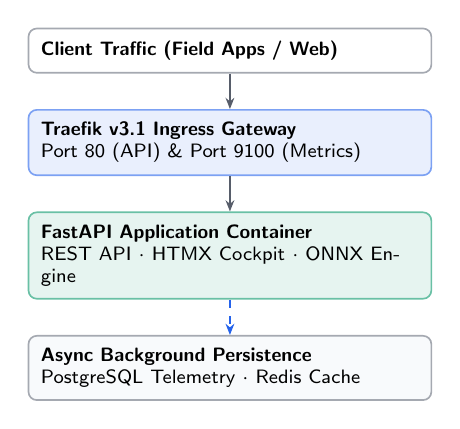
\begin{tikzpicture}[node distance=0.45cm]
                \node[nodecard, text width=4.8cm, fill=white] (user) {\textbf{Client Traffic (Field Apps / Web)}};
                \node[nodecard, draw=BlueAccent!60, fill=BlueAccent!10, text width=4.8cm, below=of user] (traefik) {\textbf{Traefik v3.1 Ingress Gateway}\\\scriptsize Port 80 (API) \& Port 9100 (Metrics)};
                \node[nodecard, draw=GreenAccent!60, fill=GreenAccent!10, text width=4.8cm, below=of traefik] (app) {\textbf{FastAPI Application Container}\\\scriptsize REST API $\cdot$ HTMX Cockpit $\cdot$ ONNX Engine};
                \node[nodecard, text width=4.8cm, below=of app] (pg) {\textbf{Async Background Persistence}\\\scriptsize PostgreSQL Telemetry $\cdot$ Redis Cache};
                
                \draw[flowarrow] (user) -- (traefik);
                \draw[flowarrow] (traefik) -- (app);
                \draw[dasharrow] (app) -- (pg);
            \end{tikzpicture}
        \end{column}
    \end{columns}
\end{frame}

% ==============================================================================
% SLIDE 17: Telemetry & Database Feature Persistence
% ==============================================================================
\begin{frame}{Telemetry \& Database Feature Persistence}{Asynchronous PostgreSQL Ingestion Without Serving Latency Penalty}
    \begin{columns}[T]
        \begin{column}{0.50\textwidth}
            \begin{bluecard}
                \textbf{\color{BlueAccent} Why We Persist Embeddings in Production}\\[3pt]
                \textbullet\ Detecting representation shift requires analysing feature representations from live traffic.\\[2pt]
                \textbullet\ Storing raw photos would exhaust storage and violates user privacy.\\[2pt]
                \textbullet\ Instead, TaxonVision persists the \textbf{384-dimensional feature vector} (\texttt{embedding REAL[]}) directly in PostgreSQL.\\[2pt]
                \textbullet\ \textbf{Event Loop Protection (Rule 08):} Written asynchronously via \texttt{BackgroundTasks} -- request returns in $18\,\text{ms}$ while I/O runs in background.
            \end{bluecard}
        \end{column}
        \begin{column}{0.46\textwidth}
            \begin{card}
                \textbf{\color{SlateDark} Telemetry Schema (\texttt{predictions} table)}\\[2pt]
                \textbullet\ \texttt{observation\_id} (UUID primary key)\\
                \textbullet\ \texttt{created\_at} (Timestamptz index)\\
                \textbullet\ \texttt{top1\_taxon} \& \texttt{top1\_confidence}\\
                \textbullet\ \texttt{conformal\_set} (\texttt{TEXT[]} array)\\
                \textbullet\ \texttt{ood\_energy} \& \texttt{is\_ood} (Boolean)\\
                \textbullet\ \texttt{latency\_ms} (Measured wall-clock)\\
                \textbullet\ \textbf{\texttt{embedding} (\texttt{REAL[]}, 384 dimensions)}\\[2pt]
                \scriptsize Ready for instantaneous sliding-window drift queries!
            \end{card}
        \end{column}
    \end{columns}
\end{frame}

% ==============================================================================
% SLIDE 18: Automated Representation Drift Detection
% ==============================================================================
\begin{frame}{Automated Drift Detection in Practice}{Evidently AI Reports \& Two-Tier Hypothesis Testing}
    \begin{columns}[T]
        \begin{column}{0.48\textwidth}
            \begin{bluecard}
                \textbf{\color{BlueAccent} Two-Tier Drift Evaluation Engine}\\[2pt]
                \textbullet\ \textbf{Tier 1: Wasserstein-1 ($W_1$) on Norms}\\[1pt]
                \quad Fast linear-time check on embedding lengths; catches immediate camera/contrast shift.\\[2pt]
                \textbullet\ \textbf{Tier 2: Kernel MMD² Permutation Test}\\[1pt]
                \quad Multivariate distribution test ($B=200$); detects subtle manifold distortion ($p < 0.01$).\\[2pt]
                \textbullet\ \textbf{Evidently AI 0.7 HTML Dashboard:}\\[1pt]
                \quad Projects 384 dims to 8 PCA components and renders interactive reports (\texttt{drift\_report.html}).
            \end{bluecard}
        \end{column}
        \begin{column}{0.48\textwidth}
            \begin{greencard}
                \textbf{\color{GreenAccent} Automated MLflow Tracking Lineage}\\[2pt]
                \textbullet\ Evaluated hourly by the Airflow DAG \texttt{prediction\_drift\_monitor}.\\[2pt]
                \textbullet\ Automatically creates an MLflow run in experiment \texttt{taxon-vision-drift}.\\[2pt]
                \textbullet\ Logs metrics (\texttt{drift\_w1}, \texttt{drift\_mmd2}, \texttt{p\_value}), tag \texttt{drift\_detected=true/false}.\\[2pt]
                \textbullet\ Attaches the Evidently HTML dashboard as an immutable build artefact.
            \end{greencard}
        \end{column}
    \end{columns}
\end{frame}

% ==============================================================================
% SLIDE 19: Prometheus & Grafana Observability Cockpit
% ==============================================================================
\begin{frame}{Prometheus \& Grafana Observability Cockpit}{Real-Time Operational Monitoring and Four Alerting Rules}
    \begin{columns}[T]
        \begin{column}{0.48\textwidth}
            \begin{ambercard}
                \textbf{\color{AmberAccent} Real-Time Metrics \& Dashboards}\\[2pt]
                \textbullet\ \textbf{Prometheus Pull Scraper:} Scrapes \texttt{/metrics} every 15 seconds across serving and Traefik pods.\\[2pt]
                \textbullet\ \textbf{Grafana Cockpit (6 Panels):}
                \begin{itemize}\scriptsize
                    \item Request rate and status codes (2xx, 4xx, 5xx).
                    \item p50, p95, p99 end-to-end latency histograms.
                    \item Conformal set size distribution.
                    \item Human triage referral rate.
                    \item Live drift distance gauge ($W_1$).
                \end{itemize}
            \end{ambercard}
        \end{column}
        \begin{column}{0.48\textwidth}
            \begin{rosecard}
                \textbf{\color{RoseAccent} Four Production Alerting Rules}\\[2pt]
                \textbullet\ \textbf{\texttt{PredictionLatencyP95High}:}\\
                \quad p95 latency $> 120\,\text{ms}$ for 5 min (\texttt{warning}).\\[2pt]
                \textbullet\ \textbf{\texttt{PredictionErrorRatioHigh}:}\\
                \quad Error ratio $> 5\%$ for 5 min (\texttt{critical}).\\[2pt]
                \textbullet\ \textbf{\texttt{EmbeddingDriftDetected}:}\\
                \quad Drift gauge $> 0.5$ (\texttt{critical}, \textbf{action: retrain}).\\[2pt]
                \textbullet\ \textbf{\texttt{DriftMonitorStale}:}\\
                \quad No drift run in $> 2$ hours (\texttt{warning}).
            \end{rosecard}
        \end{column}
    \end{columns}
\end{frame}

% ==============================================================================
% SLIDE 20: Closed-Loop Retraining: Grafana Webhook to Airflow
% ==============================================================================
\begin{frame}{Closed-Loop Retraining Trigger}{Grafana Alert Webhook $\to$ FastAPI Relay $\to$ Airflow 3.0 DAG}
    \centering
    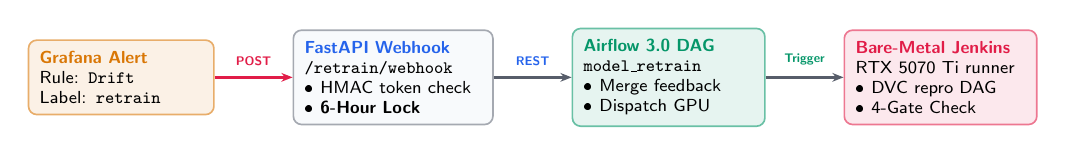
\begin{tikzpicture}[
        scale=0.90, every node/.style={transform shape},
        node distance=0.4cm and 1.1cm
    ]
        \node[nodecard, draw=AmberAccent!60, fill=AmberAccent!10, text width=2.3cm] (graf) {
            \textbf{\color{AmberAccent} Grafana Alert}\\
            \scriptsize Rule: \texttt{Drift}\\
            Label: \texttt{retrain}
        };
        
        \node[nodecard, text width=2.5cm, right=of graf] (relay) {
            \textbf{\color{BlueAccent} FastAPI Webhook}\\
            \scriptsize \texttt{/retrain/webhook}\\
            \textbullet\ HMAC token check\\
            \textbullet\ \textbf{6-Hour Lock}
        };
        
        \node[nodecard, draw=GreenAccent!60, fill=GreenAccent!10, text width=2.4cm, right=of relay] (air) {
            \textbf{\color{GreenAccent} Airflow 3.0 DAG}\\
            \scriptsize \texttt{model\_retrain}\\
            \textbullet\ Merge feedback\\
            \textbullet\ Dispatch GPU
        };
        
        \node[nodecard, draw=RoseAccent!60, fill=RoseAccent!10, text width=2.4cm, right=of air] (jenk) {
            \textbf{\color{RoseAccent} Bare-Metal Jenkins}\\
            \scriptsize RTX 5070 Ti runner\\
            \textbullet\ DVC repro DAG\\
            \textbullet\ 4-Gate Check
        };
        
        \draw[retrainarrow] (graf.east) -- (relay.west) 
            node[midway, above=1pt, font=\tiny\bfseries\color{RoseAccent}] {POST};
        \draw[flowarrow] (relay.east) -- (air.west) 
            node[midway, above=1pt, font=\tiny\bfseries\color{BlueAccent}] {REST};
        \draw[flowarrow] (air.east) -- (jenk.west) 
            node[midway, above=1pt, font=\tiny\bfseries\color{GreenAccent}] {Trigger};
    \end{tikzpicture}
    
    \vspace{0.35cm}
    \begin{bluecard}
        \centering
        \textbf{Anti-Alert-Storm Cooldown Protection:} When sudden environmental drift causes continuous alerting, the atomic 6-hour cooldown window ensures the GPU cluster executes only one retraining run, preventing resource exhaustion.
    \end{bluecard}
\end{frame}

% ==============================================================================
% SLIDE 21: Human-in-the-Loop Active Learning (Label Studio)
% ==============================================================================
\begin{frame}{Human-in-the-Loop Active Learning}{Turning Uncertain Predictions into Retraining Fuel}
    \begin{columns}[T]
        \begin{column}{0.50\textwidth}
            \begin{purplecard}
                \textbf{\color{PurpleAccent} The Closed-Loop Curation Lifecycle}\\[2pt]
                \textbullet\ \textbf{1. Epistemic Triage:} Ambiguous sets ($|C| > 3$) and empty sets ($|C| = 0$) are saved to \texttt{data/flagged\_observations/}.\\[2pt]
                \textbullet\ \textbf{2. Taxonomist Review:} Taxonomists inspect specimen crops and CAM attribution heatmaps in Label Studio.\\[2pt]
                \textbullet\ \textbf{3. Feedback Export:} Label Studio exports verified JSON multi-class annotations.\\[2pt]
                \textbullet\ \textbf{4. Airflow Ingestion:} The \texttt{model\_retraining} DAG merges feedback, validates open licences, and updates the DVC manifest.
            \end{purplecard}
        \end{column}
        \begin{column}{0.46\textwidth}
            \centering
            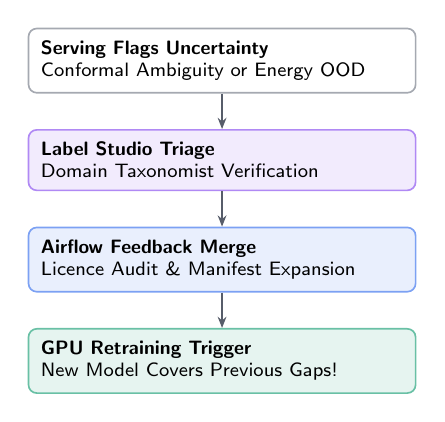
\begin{tikzpicture}[node distance=0.45cm]
                \node[nodecard, text width=4.6cm, fill=white] (flag) {\textbf{Serving Flags Uncertainty}\\\scriptsize Conformal Ambiguity or Energy OOD};
                \node[nodecard, draw=PurpleAccent!60, fill=PurpleAccent!10, text width=4.6cm, below=of flag] (ls) {\textbf{Label Studio Triage}\\\scriptsize Domain Taxonomist Verification};
                \node[nodecard, draw=BlueAccent!60, fill=BlueAccent!10, text width=4.6cm, below=of ls] (air) {\textbf{Airflow Feedback Merge}\\\scriptsize Licence Audit \& Manifest Expansion};
                \node[nodecard, draw=GreenAccent!60, fill=GreenAccent!10, text width=4.6cm, below=of air] (retrain) {\textbf{GPU Retraining Trigger}\\\scriptsize New Model Covers Previous Gaps!};
                
                \draw[flowarrow] (flag) -- (ls);
                \draw[flowarrow] (ls) -- (air);
                \draw[flowarrow] (air) -- (retrain);
            \end{tikzpicture}
        \end{column}
    \end{columns}
\end{frame}

% ==============================================================================
% SLIDE 22: Jenkins Bare-Metal Retraining & Four-Gate Promotion
% ==============================================================================
\begin{frame}{Four-Gate Model Promotion Verdict}{Strict Automated Quality Verification Before Production Alias}
    \begin{columns}[T]
        \begin{column}{0.48\textwidth}
            \begin{rosecard}
                \textbf{\color{RoseAccent} Why Validation Accuracy Is Not Enough}\\[3pt]
                \textbullet\ In production, a model can have great accuracy but fail latency budgets, lose conformal coverage, or degrade under INT8 quantization.\\[3pt]
                \textbullet\ TaxonVision enforces a strict \textbf{Four-Gate Promotion Verdict} in Stage 7 (\texttt{evaluate.py}) before any model receives the \texttt{@Production} tag.
            \end{rosecard}
        \end{column}
        \begin{column}{0.50\textwidth}
            \begin{card}
                \textbf{\color{SlateDark} The Four Automated Promotion Gates}\\[2pt]
                \textbf{Gate 1: Predictive Superiority}\\
                \textbullet\ Validation Macro PR-AUC $\ge$ active production baseline.\\[2pt]
                \textbf{Gate 2: Quantization Fidelity}\\
                \textbullet\ INT8 accuracy drop $\le 3.0\%$ relative to FP32 baseline.\\[2pt]
                \textbf{Gate 3: Empirical Conformal Coverage}\\
                \textbullet\ Holdout test coverage $\ge 90.0\%$ (nominal $95\%$).\\[2pt]
                \textbf{Gate 4: Latency Ceiling \& Exchangeability}\\
                \textbullet\ CPU p95 latency $\le 120\,\text{ms}$ and live MMD $p \ge 0.01$.
            \end{card}
        \end{column}
    \end{columns}
\end{frame}

% ==============================================================================
% SLIDE 23: CI/CD Quality Gates & Dual DVC Push
% ==============================================================================
\begin{frame}{CI/CD Quality Gates \& Dual DVC Push}{Dual-Target Toolchain: Fast CPU Gates and Headless GPU Execution}
    \begin{columns}[T]
        \begin{column}{0.48\textwidth}
            \begin{bluecard}
                \textbf{\color{BlueAccent} Pull Request Gatekeeper (GitHub Actions)}\\[3pt]
                \textbullet\ \textbf{Zero-Cost CPU Verification:}\\
                \quad Strict MyPy type checking (\texttt{mypy --strict}).\\
                \quad Ruff linting and formatting.\\
                \quad 203 unit tests with coverage threshold.\\
                \quad OKF v0.2 documentation conformance.\\
                \quad Rule 07 Hardware invariant validation.\\[2pt]
                \textbullet\ Runs on every PR before merge to \texttt{develop}.
            \end{bluecard}
        \end{column}
        \begin{column}{0.48\textwidth}
            \begin{greencard}
                \textbf{\color{GreenAccent} Heavy GPU Runner (Jenkins on Bare-Metal)}\\[3pt]
                \textbullet\ Executes DVC pipeline on NVIDIA RTX 5070 Ti.\\[2pt]
                \textbullet\ \textbf{Dual DVC Push Sequence:}
                \begin{itemize}\scriptsize
                    \item \texttt{dvc push -r local-seaweedfs}: In-cluster NVMe S3 update for immediate serving volume mount.
                    \item \texttt{dvc push -r origin}: DagsHub Cloud S3 sync for persistent public archiving.
                \end{itemize}
                \textbullet\ \textbf{Automated Git Lineage:} Commits updated \texttt{dvc.lock} and metrics back to repository.
            \end{greencard}
        \end{column}
    \end{columns}
\end{frame}

% ==============================================================================
% SLIDE 24: Summary & Core Architecture Achievements
% ==============================================================================
\begin{frame}{Summary \& Core Architecture Achievements}{Phase 1, 2, and 3 Successfully Delivered}
    \begin{columns}[T]
        \begin{column}{0.32\textwidth}
            \begin{bluecard}
                \centering
                \textbf{\color{BlueAccent} 1. Robust MLOps}\\[3pt]
                \scriptsize
                \textbullet\ 7-Stage DVC Pipeline\\
                \textbullet\ Dual-Tier S3 Remote\\
                \textbullet\ MLflow 3.x Registry\\
                \textbullet\ Pure Pixi Toolchain\\
                \textbullet\ GPG-Signed Commits
            \end{bluecard}
        \end{column}
        \begin{column}{0.32\textwidth}
            \begin{greencard}
                \centering
                \textbf{\color{GreenAccent} 2. Speed \& Safety}\\[3pt]
                \scriptsize
                \textbullet\ Sub-15ms INT8 ONNX\\
                \textbullet\ 95\% Coverage Guarantee\\
                \textbullet\ Helmholtz Energy Filter\\
                \textbullet\ Unified FastAPI/HTMX\\
                \textbullet\ Forward Grad-CAM CAM
            \end{greencard}
        \end{column}
        \begin{column}{0.32\textwidth}
            \begin{purplecard}
                \centering
                \textbf{\color{PurpleAccent} 3. Closed Loop}\\[3pt]
                \scriptsize
                \textbullet\ Postgres Embeddings\\
                \textbullet\ Evidently 0.7 Drift\\
                \textbullet\ Grafana Webhook Relay\\
                \textbullet\ Label Studio Active Learn\\
                \textbullet\ 4-Gate Auto Retraining
            \end{purplecard}
        \end{column}
    \end{columns}
    
    \vspace{0.4cm}
    \begin{card}
        \centering
        \textbf{Key Takeaway:} TaxonVision demonstrates that production machine learning is not about training a model once in a notebook; it is about building a self-monitoring, self-healing, mathematically safe engineering loop.
    \end{card}
\end{frame}

% ==============================================================================
% SLIDE 25: Live Demonstration & Q&A
% ==============================================================================
\begin{frame}[plain]
    \vspace{0.5cm}
    \begin{center}
        {\Huge\bfseries\color{SlateDark} Live Demonstration \& Q\&A}\\[6pt]
        {\large\color{BlueAccent} Real-Time Inference $\cdot$ Conformal Sets $\cdot$ Observability Cockpit}
        
        \vspace{0.6cm}
        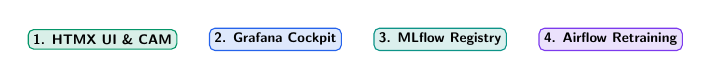
\begin{tikzpicture}[node distance=0.4cm]
            \node[pill, fill=GreenAccent!15, draw=GreenAccent] (demo1) {\textbf{1. HTMX UI \& CAM}};
            \node[pill, fill=BlueAccent!15, draw=BlueAccent, right=of demo1] (demo2) {\textbf{2. Grafana Cockpit}};
            \node[pill, fill=TealAccent!15, draw=TealAccent, right=of demo2] (demo3) {\textbf{3. MLflow Registry}};
            \node[pill, fill=PurpleAccent!15, draw=PurpleAccent, right=of demo3] (demo4) {\textbf{4. Airflow Retraining}};
        \end{tikzpicture}
        
        \vspace{0.8cm}
        {\small\textbf{Thank you for your attention!}}\\[2pt]
        {\footnotesize\color{TextMuted} We now transition to the live system demonstration and jury questions.}
    \end{center}
\end{frame}

\end{document}
